% Drawing 121/03-1 -- folder 121, batch 03, archive page 44 (PDF page 45).
% Transcription: page de dessins : une suite de figures numérotées 1°) à 6°) (un point $U_0$, puis $U_0$ et $U_0'$, des « haltères », des régions hachurées $V^{\circ\prime}$, $U''$), marquées I et II. En haut, la tour $U_0 \subset U_1 \subset U_2 \subset U_3 \ldots U_n$, avec $U_1^{\circ}$, $U_2^{\circ}$, $U_3^{\circ}$, $\partial U_1^{\circ} = U_0'$, $\partial U_2^{\circ}$, $U_1^{\circ\prime}$, $U_0''$, $\partial U_1^{\circ\prime} = \partial U''$, $U_2^{\circ\prime}$, $\partial U_2^{\circ\prime}$. À droite, un schéma vertical :
% Kind: page of drawings: tower U_0 in U_1 in ..., boundary scheme, dumbbells, regions I and II, figures 1o)-6o). Method 2 (schematic redraw from the facsimile). Status: partial.
% Notes: Whole sheet, at 2 mm per unit with the labels at \small. Top left, the tower U_0 in U_1 in U_2, U_3 with U_i^o, their boundaries, U_1^o', U_0'', U_2^o' and the arrows (curved arrows approximate); top right the vertical scheme U_n -> U_n^o <- dU_n^o -> d_{n-1}U_n^o, ..., d_0U_n^o -> U_{n-1}^o, ..., U_0^o = U_0. Left column: the two dumbbells are redrawn on a tight crop: the first with its two rings open towards the bars, the two outer bars ending on the rings and the heavy bar between the two points; the second with its three bars ending on the two (hatched) rings and the two strokes from the points down to the apex, with two points on them; then a triangle, two segments, a small knob on three lines, and the large figure with U'', V^o, V^o', U' (hatched bar). Right: a dumbbell with strokes marked I and II inside a large pencil circle, a hatched fan, and the numbered sequence 1o)-6o) (U_0, U_0', U_1^o, hatched regions), schematised; many of its small labels are left out. An ink blot at the left is not drawn. Still differs (kept from the earlier redraw, overlay off by 1 to 3 units): the dumbbell with I and II and its pencil circle, the rings of the U'' figure (drawn too large), the hatched fans and the sequence 1o)-6o), whose many small labels U_0', U_1^o are left out. Redrawn 2026-11-09 (issue 128): to check again.
% Coordinates: 1 unit = 2 mm = 1/100 of the crop width (bbox in page fractions: [0.04, 0.04, 0.97, 0.88]).
% Redrawn by Claude (claude-opus-5-5), issue #73, 2026-11-09; not checked by a human; not compiled (no TeX in the session).
% Rights: reproduces part of the work -- behind RENDER_TRANSCRIPTS, never published by itself.
\documentclass[tikz,border=3pt]{standalone}
\usepackage{amsmath,amssymb}
\usetikzlibrary{patterns,arrows.meta}
\tikzset{pencil/.style={black!45}, struck/.style={black!35}, mark/.style={circle,draw,inner sep=1.3pt}, pt/.style={circle,fill,inner sep=0.9pt}, opt/.style={circle,draw,fill=white,inner sep=1.1pt}}
\begin{document}
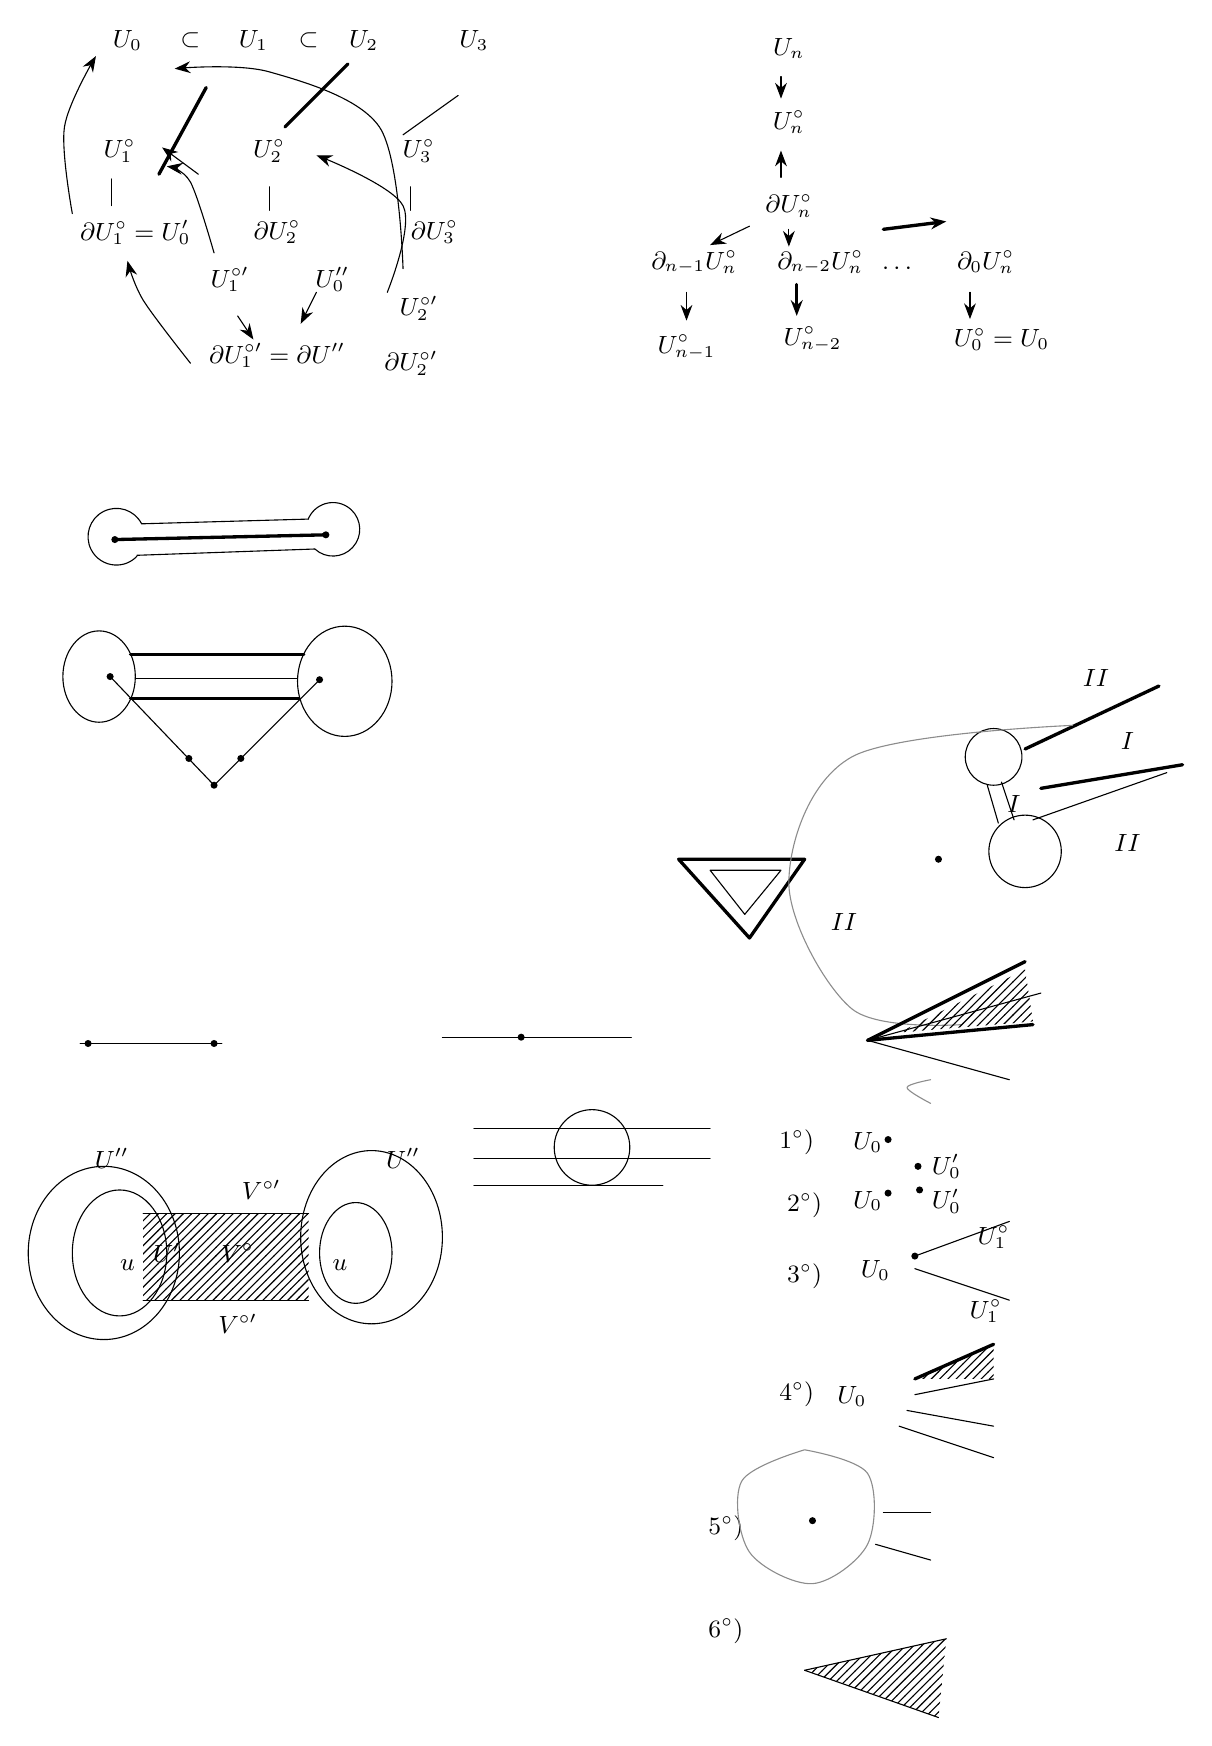
\begin{tikzpicture}[x=2mm,y=2mm,line cap=round,line join=round,font=\scriptsize]
\node[inner sep=1pt] at (19,-16.5) {\small $U_0$};
\node[inner sep=1pt] at (23,-16.5) {\small $\subset$};
\node[inner sep=1pt] at (27,-16.5) {\small $U_1$};
\node[inner sep=1pt] at (30.5,-16.5) {\small $\subset$};
\node[inner sep=1pt] at (34,-16.5) {\small $U_2$};
\node[inner sep=1pt] at (41,-16.5) {\small $U_3$};
\node[inner sep=1pt] at (18.5,-23.5) {\small $U_1^\circ$};
\node[inner sep=1pt] at (28,-23.5) {\small $U_2^\circ$};
\node[inner sep=1pt] at (37.5,-23.5) {\small $U_3^\circ$};
\draw (18,-25.3) -- (18,-27);
\draw (28,-25.8) -- (28,-27.3);
\draw (37,-25.8) -- (37,-27.3);
\node[inner sep=1pt] at (19.5,-28.7) {\small $\partial U_1^\circ=U_0'$};
\node[inner sep=1pt] at (28.5,-28.7) {\small $\partial U_2^\circ$};
\node[inner sep=1pt] at (38.5,-28.7) {\small $\partial U_3^\circ$};
\node[inner sep=1pt] at (25.5,-31.7) {\small $U_1^{\circ\prime}$};
\node[inner sep=1pt] at (32,-31.7) {\small $U_0''$};
\node[inner sep=1pt] at (37.5,-33.5) {\small $U_2^{\circ\prime}$};
\node[inner sep=1pt] at (28.5,-36.5) {\small $\partial U_1^{\circ\prime}=\partial U''$};
\node[inner sep=1pt] at (37,-37) {\small $\partial U_2^{\circ\prime}$};
\draw[-{Stealth[length=2mm]}] plot[smooth, tension=0.55] coordinates {(15.5,-27.5) (15,-22) (17,-17.5)};
\draw[-{Stealth[length=2mm]}] (23.5,-25) -- (21.2,-23.3);
\draw[very thick] (21,-25) -- (24,-19.5);
\draw[very thick] (29,-22) -- (33,-18);
\draw (40,-20) -- (36.5,-22.5);
\draw[-{Stealth[length=2mm]}] plot[smooth, tension=0.55] coordinates {(36.5,-31) (35,-22) (28,-18.5) (22,-18.3)};
\draw[-{Stealth[length=2mm]}] plot[smooth, tension=0.55] coordinates {(24.5,-30) (23,-25.5) (21.5,-24.5)};
\draw[-{Stealth[length=2mm]}] (26,-34) -- (27,-35.5);
\draw[-{Stealth[length=2mm]}] (31,-32.5) -- (30,-34.5);
\draw[-{Stealth[length=2mm]}] plot[smooth, tension=0.55] coordinates {(23,-37) (20,-33) (19,-30.5)};
\draw[-{Stealth[length=2mm]}] plot[smooth, tension=0.55] coordinates {(35.5,-32.5) (36.5,-27) (31,-23.8)};
\node[inner sep=1pt] at (61,-17) {\small $U_n$};
\draw[-{Stealth[length=2mm]}] (60.5,-18.8) -- (60.5,-20.2);
\node[inner sep=1pt] at (61,-21.7) {\small $U_n^\circ$};
\draw[{Stealth[length=2mm]}-] (60.5,-23.5) -- (60.5,-25.2);
\node[inner sep=1pt] at (61,-27) {\small $\partial U_n^\circ$};
\draw[-{Stealth[length=2mm]}] (58.5,-28.3) -- (56,-29.5);
\draw[-{Stealth[length=2mm]}] (61,-28.5) -- (61,-29.6);
\draw[-{Stealth[length=2mm]},very thick] (67,-28.5) -- (71,-28);
\node[inner sep=1pt] at (55,-30.6) {\small $\partial_{n-1}U_n^\circ$};
\node[inner sep=1pt] at (63,-30.6) {\small $\partial_{n-2}U_n^\circ$};
\node[inner sep=1pt] at (68,-31) {\small $\cdots$};
\node[inner sep=1pt] at (73.5,-30.6) {\small $\partial_0U_n^\circ$};
\draw[-{Stealth[length=2mm]}] (54.5,-32.5) -- (54.5,-34.3);
\draw[-{Stealth[length=2mm]},very thick] (61.5,-32) -- (61.5,-34);
\draw[-{Stealth[length=2mm]}] (72.5,-32.5) -- (72.5,-34.2);
\node[inner sep=1pt] at (54.5,-36) {\small $U_{n-1}^\circ$};
\node[inner sep=1pt] at (62.5,-35.5) {\small $U_{n-2}^\circ$};
\node[inner sep=1pt] at (74.5,-35.5) {\small $U_0^\circ=U_0$};
\draw[very thick] (54,-68.5) -- (62,-68.5) -- (58.5,-73.5) -- cycle;
\draw (56,-69.2) -- (60.5,-69.2) -- (58.2,-72) -- cycle;
\draw (16,-80.2) -- (25,-80.2);
\node[pt] at (16.5,-80.2) {};
\node[pt] at (24.5,-80.2) {};
\draw (39,-79.8) -- (51,-79.8);
\node[pt] at (44,-79.8) {};
\draw (48.5,-86.8) circle[radius=2.4];
\draw (41,-85.6) -- (56,-85.6);
\draw (41,-87.5) -- (56,-87.5);
\draw (41,-89.2) -- (53,-89.2);
\draw (17.5,-93.5) ellipse[x radius=4.8, y radius=5.5];
\draw (18.5,-93.5) ellipse[x radius=3, y radius=4];
\draw (34.5,-92.5) ellipse[x radius=4.5, y radius=5.5];
\draw (33.5,-93.5) ellipse[x radius=2.3, y radius=3.2];
\draw (20,-91) -- (30.5,-91);
\draw (20,-96.5) -- (30.5,-96.5);
\fill[pattern=north east lines] (20,-91) -- (30.5,-91) -- (30.5,-96.5) -- (20,-96.5) -- cycle;
\node[inner sep=1pt] at (18,-87.5) {\small $U''$};
\node[inner sep=1pt] at (36.5,-87.5) {\small $U''$};
\node[inner sep=1pt] at (27.5,-89.5) {\small $V^{\circ\prime}$};
\node[inner sep=1pt] at (26,-93.5) {\small $V^\circ$};
\node[inner sep=1pt] at (26,-98) {\small $V^{\circ\prime}$};
\node[inner sep=1pt] at (21.5,-93.5) {\small $U'$};
\node[inner sep=1pt] at (19,-94.3) {\small $u$};
\node[inner sep=1pt] at (32.5,-94.3) {\small $u$};
\draw (74,-62) circle[radius=1.8];
\draw (76,-68) circle[radius=2.3];
\draw (74.5,-63.6) -- (75.3,-66);
\draw (73.6,-63.8) -- (74.3,-66.2);
\draw[very thick] (76,-61.5) -- (84.5,-57.5);
\draw[very thick] (77,-64) -- (86,-62.5);
\draw (76.5,-66) -- (85,-63);
\node[inner sep=1pt] at (82.5,-61) {\small $I$};
\node[inner sep=1pt] at (80.5,-57) {\small $II$};
\node[inner sep=1pt] at (75.3,-65) {\small $I$};
\node[inner sep=1pt] at (82.5,-67.5) {\small $II$};
\draw[pencil] plot[smooth, tension=0.55] coordinates {(79,-60) (65,-62) (61,-70) (65,-78) (72,-79)};
\node[pt] at (70.5,-68.5) {};
\node[inner sep=1pt] at (64.5,-72.5) {\small $II$};
\draw[very thick] (66,-80) -- (76,-75);
\draw (66,-80) -- (77,-77);
\draw[very thick] (66,-80) -- (76.5,-79);
\draw (66,-80) -- (75,-82.5);
\fill[pattern=north east lines] (68,-79.5) -- (76,-75.5) -- (76.5,-78.8) -- cycle;
\draw[pencil] plot[smooth, tension=0.55] coordinates {(70,-82.5) (68.5,-83) (70,-84)};
\node[inner sep=1pt] at (61.5,-86.5) {\small $1^\circ)$};
\node[inner sep=1pt] at (66,-86.5) {\small $U_0$};
\node[pt] at (67.3,-86.3) {};
\node[pt] at (69.2,-88) {};
\node[inner sep=1pt] at (71,-88) {\small $U_0'$};
\node[inner sep=1pt] at (62,-90.5) {\small $2^\circ)$};
\node[inner sep=1pt] at (66,-90.2) {\small $U_0$};
\node[pt] at (67.3,-89.7) {};
\node[pt] at (69.3,-89.5) {};
\node[inner sep=1pt] at (71,-90.2) {\small $U_0'$};
\node[inner sep=1pt] at (62,-95) {\small $3^\circ)$};
\node[inner sep=1pt] at (66.5,-94.6) {\small $U_0$};
\node[pt] at (69,-93.7) {};
\draw (69,-93.7) -- (75,-91.5);
\draw (69,-94.5) -- (75,-96.5);
\node[inner sep=1pt] at (74,-92.5) {\small $U_1^\circ$};
\node[inner sep=1pt] at (73.5,-97.2) {\small $U_1^\circ$};
\node[inner sep=1pt] at (61.5,-102.5) {\small $4^\circ)$};
\node[inner sep=1pt] at (65,-102.6) {\small $U_0$};
\draw[very thick] (69,-101.5) -- (74,-99.3);
\draw (69,-102.5) -- (74,-101.5);
\draw (68.5,-103.5) -- (74,-104.5);
\draw (68,-104.5) -- (74,-106.5);
\fill[pattern=north east lines] (69,-101.5) -- (74,-99.3) -- (74,-101.5) -- cycle;
\node[inner sep=1pt] at (57,-111) {\small $5^\circ)$};
\draw[pencil] plot[smooth, tension=0.55] coordinates {(62,-106) (58,-108) (58.5,-112.5) (62.5,-114.5) (66,-112) (66,-107.5) (62,-106)};
\node[pt] at (62.5,-110.5) {};
\draw (67,-110) -- (70,-110);
\draw (66.5,-112) -- (70,-113);
\node[inner sep=1pt] at (57,-117.5) {\small $6^\circ)$};
\draw (62,-120) -- (71,-118);
\draw (62,-120) -- (70.5,-123);
\fill[pattern=north east lines] (62,-120) -- (71,-118) -- (70.5,-123) -- cycle;
\draw (19.9,-47.2) arc[start angle=27.1, end angle=316.6, x radius=1.8, y radius=1.8];
\draw (30.9,-48.8) arc[start angle=227.4, end angle=517.5, x radius=1.7, y radius=1.7];
\draw (19.9,-47.2) -- (30.5,-46.9);
\draw (19.6,-49.2) -- (30.9,-48.8);
\draw[very thick] (18.2,-48.2) -- (31.6,-47.9);
\node[pt] at (18.2,-48.2) {};
\node[pt] at (31.6,-47.9) {};
\draw (17.2,-56.9) ellipse[x radius=2.3, y radius=2.9];
\draw (32.8,-57.2) ellipse[x radius=3, y radius=3.5];
\draw[very thick] (19.2,-55.5) -- (30.2,-55.5);
\draw (19.5,-57) -- (29.8,-57);
\draw[very thick] (19.2,-58.3) -- (29.9,-58.3);
\draw (17.9,-56.9) -- (24.5,-63.8) -- (31.2,-57.1);
\node[pt] at (17.9,-56.9) {};
\node[pt] at (31.2,-57.1) {};
\node[pt] at (24.5,-63.8) {};
\node[pt] at (22.9,-62.1) {};
\node[pt] at (26.2,-62.1) {};
\end{tikzpicture}
\end{document}
